%%%%%%%%%%%%%%%%%%%%%%%%%%%%%%%%%%%%%%%%%
% Lachaise Assignment
% LaTeX Template
% Version 1.0 (26/6/2018)
%
% This template originates from:
% http://www.LaTeXTemplates.com
%
% Authors:
% Marion Lachaise & François Févotte
% Vel (vel@LaTeXTemplates.com)
%
% License:
% CC BY-NC-SA 3.0 (http://creativecommons.org/licenses/by-nc-sa/3.0/)
% 
%%%%%%%%%%%%%%%%%%%%%%%%%%%%%%%%%%%%%%%%%

%----------------------------------------------------------------------------------------
%	PACKAGES AND OTHER DOCUMENT CONFIGURATIONS
%----------------------------------------------------------------------------------------

\documentclass{article}

%%%%%%%%%%%%%%%%%%%%%%%%%%%%%%%%%%%%%%%%%
% Lachaise Assignment
% Structure Specification File
% Version 1.0 (26/6/2018)
%
% This template originates from:
% http://www.LaTeXTemplates.com
%
% Authors:
% Marion Lachaise & François Févotte
% Vel (vel@LaTeXTemplates.com)
%
% License:
% CC BY-NC-SA 3.0 (http://creativecommons.org/licenses/by-nc-sa/3.0/)
% 
%%%%%%%%%%%%%%%%%%%%%%%%%%%%%%%%%%%%%%%%%

%----------------------------------------------------------------------------------------
%	PACKAGES AND OTHER DOCUMENT CONFIGURATIONS
%----------------------------------------------------------------------------------------

\usepackage{amsmath,amsfonts,stmaryrd,amssymb} % Math packages

\usepackage{enumerate} % Custom item numbers for enumerations

\usepackage[ruled]{algorithm2e} % Algorithms

\usepackage[framemethod=tikz]{mdframed} % Allows defining custom boxed/framed environments

\usepackage{listings} % File listings, with syntax highlighting
\lstset{
	basicstyle=\ttfamily, % Typeset listings in monospace font
}

\usepackage[english,russian]{babel}	% локализация и переносы

\usepackage{amsfonts}

%----------------------------------------------------------------------------------------
%	DOCUMENT MARGINS
%----------------------------------------------------------------------------------------

\usepackage{geometry} % Required for adjusting page dimensions and margins

\geometry{
	paper=a4paper, % Paper size, change to letterpaper for US letter size
	top=2.5cm, % Top margin
	bottom=3cm, % Bottom margin
	left=2.5cm, % Left margin
	right=2.5cm, % Right margin
	headheight=14pt, % Header height
	footskip=1.5cm, % Space from the bottom margin to the baseline of the footer
	headsep=1.2cm, % Space from the top margin to the baseline of the header
	%showframe, % Uncomment to show how the type block is set on the page
}

%----------------------------------------------------------------------------------------
%	FONTS
%----------------------------------------------------------------------------------------

\usepackage[utf8]{inputenc} % Required for inputting international characters
\usepackage[T1]{fontenc} % Output font encoding for international characters

\usepackage{XCharter} % Use the XCharter fonts

%----------------------------------------------------------------------------------------
%	COMMAND LINE ENVIRONMENT
%----------------------------------------------------------------------------------------

% Usage:
% \begin{commandline}
	%	\begin{verbatim}
		%		$ ls
		%		
		%		Applications	Desktop	...
		%	\end{verbatim}
	% \end{commandline}

\mdfdefinestyle{commandline}{
	leftmargin=10pt,
	rightmargin=10pt,
	innerleftmargin=15pt,
	middlelinecolor=black!50!white,
	middlelinewidth=2pt,
	frametitlerule=false,
	backgroundcolor=black!5!white,
	frametitle={Command Line},
	frametitlefont={\normalfont\sffamily\color{white}\hspace{-1em}},
	frametitlebackgroundcolor=black!50!white,
	nobreak,
}

% Define a custom environment for command-line snapshots
\newenvironment{commandline}{
	\medskip
	\begin{mdframed}[style=commandline]
	}{
	\end{mdframed}
	\medskip
}

%----------------------------------------------------------------------------------------
%	FILE CONTENTS ENVIRONMENT
%----------------------------------------------------------------------------------------

% Usage:
% \begin{file}[optional filename, defaults to "File"]
	%	File contents, for example, with a listings environment
	% \end{file}

\mdfdefinestyle{file}{
	innertopmargin=1.6\baselineskip,
	innerbottommargin=0.8\baselineskip,
	topline=false, bottomline=false,
	leftline=false, rightline=false,
	leftmargin=2cm,
	rightmargin=2cm,
	singleextra={%
		\draw[fill=black!10!white](P)++(0,-1.2em)rectangle(P-|O);
		\node[anchor=north west]
		at(P-|O){\ttfamily\mdfilename};
		%
		\def\l{3em}
		\draw(O-|P)++(-\l,0)--++(\l,\l)--(P)--(P-|O)--(O)--cycle;
		\draw(O-|P)++(-\l,0)--++(0,\l)--++(\l,0);
	},
	nobreak,
}

% Define a custom environment for file contents
\newenvironment{file}[1][File]{ % Set the default filename to "File"
	\medskip
	\newcommand{\mdfilename}{#1}
	\begin{mdframed}[style=file]
	}{
	\end{mdframed}
	\medskip
}

%----------------------------------------------------------------------------------------
%	NUMBERED QUESTIONS ENVIRONMENT
%----------------------------------------------------------------------------------------

% Usage:
% \begin{question}[optional title]
	%	Question contents
	% \end{question}

\mdfdefinestyle{question}{
	innertopmargin=1.2\baselineskip,
	innerbottommargin=0.8\baselineskip,
	roundcorner=5pt,
	nobreak,
	singleextra={%
		\draw(P-|O)node[xshift=1em,anchor=west,fill=white,draw,rounded corners=5pt]{%
			Question \theQuestion\questionTitle};
	},
}

\newcounter{Question} % Stores the current question number that gets iterated with each new question

% Define a custom environment for numbered questions
\newenvironment{question}[1][\unskip]{
	\bigskip
	\stepcounter{Question}
	\newcommand{\questionTitle}{~#1}
	\begin{mdframed}[style=question]
	}{
	\end{mdframed}
	\medskip
}

%----------------------------------------------------------------------------------------
%	WARNING TEXT ENVIRONMENT
%----------------------------------------------------------------------------------------

% Usage:
% \begin{warn}[optional title, defaults to "Warning:"]
	%	Contents
	% \end{warn}

\mdfdefinestyle{warning}{
	topline=false, bottomline=false,
	leftline=false, rightline=false,
	nobreak,
	singleextra={%
		\draw(P-|O)++(-0.5em,0)node(tmp1){};
		\draw(P-|O)++(0.5em,0)node(tmp2){};
		\fill[black,rotate around={45:(P-|O)}](tmp1)rectangle(tmp2);
		\node at(P-|O){\color{white}\scriptsize\bf !};
		\draw[very thick](P-|O)++(0,-1em)--(O);%--(O-|P);
	}
}

% Define a custom environment for warning text
\newenvironment{warn}[1][Warning:]{ % Set the default warning to "Warning:"
	\medskip
	\begin{mdframed}[style=warning]
		\noindent{\textbf{#1}}
	}{
	\end{mdframed}
}

%----------------------------------------------------------------------------------------
%	INFORMATION ENVIRONMENT
%----------------------------------------------------------------------------------------

% Usage:
% \begin{info}[optional title, defaults to "Info:"]
	% 	contents
	% 	\end{info}

\mdfdefinestyle{info}{%
	topline=false, bottomline=false,
	leftline=false, rightline=false,
	nobreak,
	singleextra={%
		\fill[black](P-|O)circle[radius=0.4em];
		\node at(P-|O){\color{white}\scriptsize\bf i};
		\draw[very thick](P-|O)++(0,-0.8em)--(O);%--(O-|P);
	}
}

% Define a custom environment for information
\newenvironment{info}[1][Информация:]{ % Set the default title to "Info:"
	\medskip
	\begin{mdframed}[style=info]
		\noindent{\textbf{#1}}
	}{
	\end{mdframed}
}

%----------------------------------------------------------------------------------------
%           SECTION
%----------------------------------------------------------------------------------------

\usepackage{titlesec} % Allows customization of titles
\renewcommand\thesection{\Roman{section}} % Roman numerals for the sections
\renewcommand\thesubsection{\roman{subsection}} % roman numerals for subsections
\titleformat{\section}[block]{\large\scshape\centering}{\thesection.}{1em}{} % Change the look of the section titles
\titleformat{\subsection}[block]{\large}{\thesubsection.}{1em}{} % Change the look of the section titles

%----------------------------------------------------------------------------------------
%          HYPERREF
%----------------------------------------------------------------------------------------
\usepackage{hyperref}
\hypersetup{
	colorlinks=true,
	linkcolor=blue,
	filecolor=magenta,      
	urlcolor=cyan,
}


\usepackage{graphicx}

% Here: H option for float placement
\usepackage{float}

% caption and subcaption work together
\usepackage{subcaption} % loads the caption package % Include the file specifying the document structure and custom commands

%----------------------------------------------------------------------------------------
%	ASSIGNMENT INFORMATION
%----------------------------------------------------------------------------------------

\title{Методы оптимизации в машинном обучении \\ Практическое задание \#1} % Title of the assignment

\author{Рожин Андрей} % Author name

\date{НИУ ВШЭ --- \today} % University, school and/or department name(s) and a date

%----------------------------------------------------------------------------------------

\begin{document}
	
	\maketitle % Print the title
	
	%----------------------------------------------------------------------------------------
	%	INTRODUCTION
	%----------------------------------------------------------------------------------------
	
	\section*{Вступление} % Unnumbered section
	Решение задач оптимизации, является неотъемлемой частью машинного обучения. В этом документе обсуждаются базовые подходы к решению задач этого типа, а также проведение и анализ экспериментов и аналитический вывод формулы логистической регрессии в матричном виде.
	
	% Math equation/formula
	\begin{equation}
		L(w) = - \frac{1}{m} \sum\limits_{i=1}^m \biggl[y_i log\biggl(\frac{1}{1 + e^{-w^Tx_i}}\biggr) + (1 - y_i) log\biggl(1 - \frac{1}{1 + e^{-w^Tx_i}}\biggr)\biggr] + \frac{\lambda}{2} \|w\|^2
	\end{equation}
	
	Рекомендуется ознакомиться с выкладкой ниже.
	
	\begin{info} % Information block
		\\
		Документ оформлен согласно  \href{https://clck.ru/h2bZh}{этому заданию}.\\ 
		Краткое содержание задания: \\
		1. Алгоритм cпуска.
		
		1.1 Общая концепция
		
		1.2 Критерий остановки
		
		1.3 Линейный поиск - условие \textit{Армихо}, сильное условие \textit{Вульфа}.
		
		1.4 Градиентный спуск.
		
		1.5 Метод Ньютона
		
		1.6 Оптимизация вычислений \\
		2. Модели
		
		2.1 Двухклассовая логистическая регрессия.
		
		2.2. Разностная проверка градиента и гессиана \\
		3. Эксперименты.
		
		3.1 Оценка реализованных алгоритмов.		
	\end{info}
	
	%----------------------------------------------------------------------------------------
	%	PROBLEM 1
	%----------------------------------------------------------------------------------------
	
	\section{Двухклассовая логистическая регрессия} % Numbered section
	
	\begin{minipage}{0.5\textwidth}
		Прежде чем начать работу, следует ввести некоторые обозначения, которые будут использоваться в дальнейшем. Все они должны быть привычными, используемыми постоянно в теоретических выкладках.
	\end{minipage}
	\begin{minipage}{0.5\textwidth}
		\begin{flushright}
			$w$ - вектор весов объекта \\
			$x$ - матрица значений признаков объектов \\
			$y$ - истинная целевая переменная \\
			$m$ - кол-во объектов \\
			$L(w)$ - функционал ошибки
		\end{flushright}
	\end{minipage}
	
	%------------------------------------------------
	
	\subsection{Градиент}
	
	Так как мы решаем задачу бинарной классификации, то множество значений, которые принимает целевая переменная $y$ состоит из 2 цифр --- \{1, 0\}. Это очень важный элемент, которые мы будем использовать в дальнейшем, поэтому стоит его запомнить. В формуле (1) заметим сигмоидную функцию, которая дает вероятность класса. Введем функцию.
	
	\newpage
	\begin{equation}
		g(z) = \frac{1}{z + e^{-z}} 
	\end{equation}

	\begin{equation*}
		h_w(x) = g(w^Tx) = \frac{1}{z + e^{-z}}
	\end{equation*}
	
	\begin{center}
		Функция (2) обладает следующими свойствами, которые нетрудно доказать.
	\end{center}
	
	
	\begin{equation*}
		g\prime(z) = g(z)(1 - g(z))
	\end{equation*}
	
	\vspace{-0.5cm}
	\begin{equation*}
		g(-z) = 1 - g(z)
	\end{equation*}

	\begin{center}
		Перепишем функцию (1), используя новые обозначения
	\end{center}

	\begin{equation}
		L(w) = \frac{1}{m} \sum\limits_{i=1}^m \biggl[y_i log(g(w^Tx)) + (1 - y_i) log(1 - g(w^Tx))\biggr] + \frac{\lambda}{2} \|w\|^2
	\end{equation}
	
	Используя эти обозначения и свойства сигмоидной функции, приступим к нахождению производной. Предположим, что у нас есть только один объект с вектором признаков $x_i$ и одно значение целевой переменной $y_i$. Продифференцируем функцию (3) по $j$-тому значению вектора весов $w$. Дифференцировать будем без члена регуляризации, допишем его позднее.
	
	\begin{equation*}
		\frac{\partial}{\partial w_j} L(w) = - \biggl[\frac{y_i}{g(w^Tx)} - (1 - y_i)\biggl(\frac{1}{1 - g(w^Tx)}\biggr)\biggr] \frac{\partial g(w^Tx)}{\partial w_j} = 
	\end{equation*}

	\begin{equation*}
		 = - \biggl[\frac{y_i}{g(w^Tx)} - (1 - y_i)\biggl(\frac{1}{1 - g(w^Tx)}\biggr)\biggr] g(w^Tx) (1 - g(w^Tx)) \frac{\partial w^Tx}{\partial w_j} = 
	\end{equation*}

	\begin{equation*}
		= - \bigl[y_i - y_i g(w^Tx) - g(w^Tx) + y_i g(w^Tx)\bigr] x_j = 
	\end{equation*}

	\begin{equation*}
		= \bigl[h_w(x) - y_i\bigr] x_j
	\end{equation*}

	\begin{center}
		Для случая из $m$ объектов получим:
	\end{center}

	\begin{equation}
		\frac{\partial}{\partial w_j} L(w) = \frac{1}{m} \sum\limits_{i=1}^m \bigl[h_w(x_i) - y_i\bigr] x_{ij}
	\end{equation}

	Введем новые обозначения в терминах векторов и матриц.
	
	\vspace{0.3cm}
	\begin{minipage}{0.5\textwidth}
		\begin{flushleft}
			$X \in \mathbb{R}^{m \times n} $ --- матрица объекты-признаки
			$y \in \mathbb{R}^{m \times 1} $ --- вектор целевых переменных
			$w \in \mathbb{R}^{1 \times n} $ --- вектор весов
		\end{flushleft}
	\end{minipage}

	Используя эти обозначения введем матричное представление функции (4)
	
	\begin{equation*}
		\nabla L(w) = \frac{1}{m} X^T \bigl[g(Xw) - y\bigr]
	\end{equation*}

	Добавим член регуляризации и получим формулу (5).
	
	\begin{equation}
		\nabla L(w) = \frac{1}{m} X^T \bigl[g(Xw) - y\bigr] + \lambda w
	\end{equation}
	
	Сам функционал логистической регрессии, формула (1), можно представить в такой матричной форме.
	
	\begin{equation}
		L(w) = -\frac{1}{m} (1, 1, ... , 1) log\bigl(-(2y-1) \circ g(Xw)\bigr)  + \frac{\lambda}{2} \|w\|^2
	\end{equation}

	\newpage
	\subsection{Гессиан}
	
	Выше мы получили функцию (4). Теперь снова продифференцируем ее, в предположении, что у нас один объект в выборке и нет регуляризации.
	
	\begin{equation}
		\frac{\partial}{\partial w_j \partial w_j^T} L(w) = \frac{\partial}{\partial w_j^T} \bigl[g(w^Tx_i) - y_i\bigr] x_i =  x_i x_i^T g(w^Tx_i) (1 - g(w^Tx_i))
	\end{equation}
	
	Для $m$ объектов и регуляризации формула(7) выглядит так:
	
	
	\begin{equation}
		\nabla^2 L(w) = \frac{1}{m} \sum\limits_{i=1}^m \biggl[x_i x_i^T g(w^Tx_i) (1 - g(w^Tx_i)) \biggr] - \lambda I
	\end{equation}

	Заметим, что матрицу $g(w^Tx_i) (1 - g(w^Tx_i))$ можно заменить диагональной матрицей, на главной диагонали которой, будут располагаться элементы $g(w^Tx_i) (1 - g(w^Tx_i))$. Назовем эту диагональную матрицу буквой $Z$.
	
	\vspace{0.5cm}
	Таким образом, мы получаем матричную форму функции (8).
	
	\begin{equation}
		\nabla^2 L(w) = \frac{1}{m} X^T Z X - \lambda I
	\end{equation}
	
	\vspace{2cm}
	
	\section{Эксперименты}
	
	В этой главе мы приступим к оценке реализованных алгоритмов градиентного спуска. Начнем с анализа вариантов линейного поиска шага и закончим логистической регрессией. 
	
	\subsection{Траектория градиентного спуска на квадратичной функции}
	
	Начнем с {\it двумерной} квадратичной функции $f(w) = \frac{1}{2} \langle Xw, w \rangle  - \langle y, w \rangle $, где $X \in \mathbb{S}_{++}^n$, $b \in \mathbb{R}^n$. Придумаем 4 функции, поведения спуска на которых, будет отличаться.
	
	\vspace{0.5cm}
	{\bf Обусловленность.} Проанализируем графики ниже.

	\begin{figure}[H]
		\centering
		\subcaptionbox{$X =  \left( \begin{smallmatrix} 1 & 0\\ 0 & 50 \end{smallmatrix}  \right)$, $w_0 = (10.0, 4.0)$}{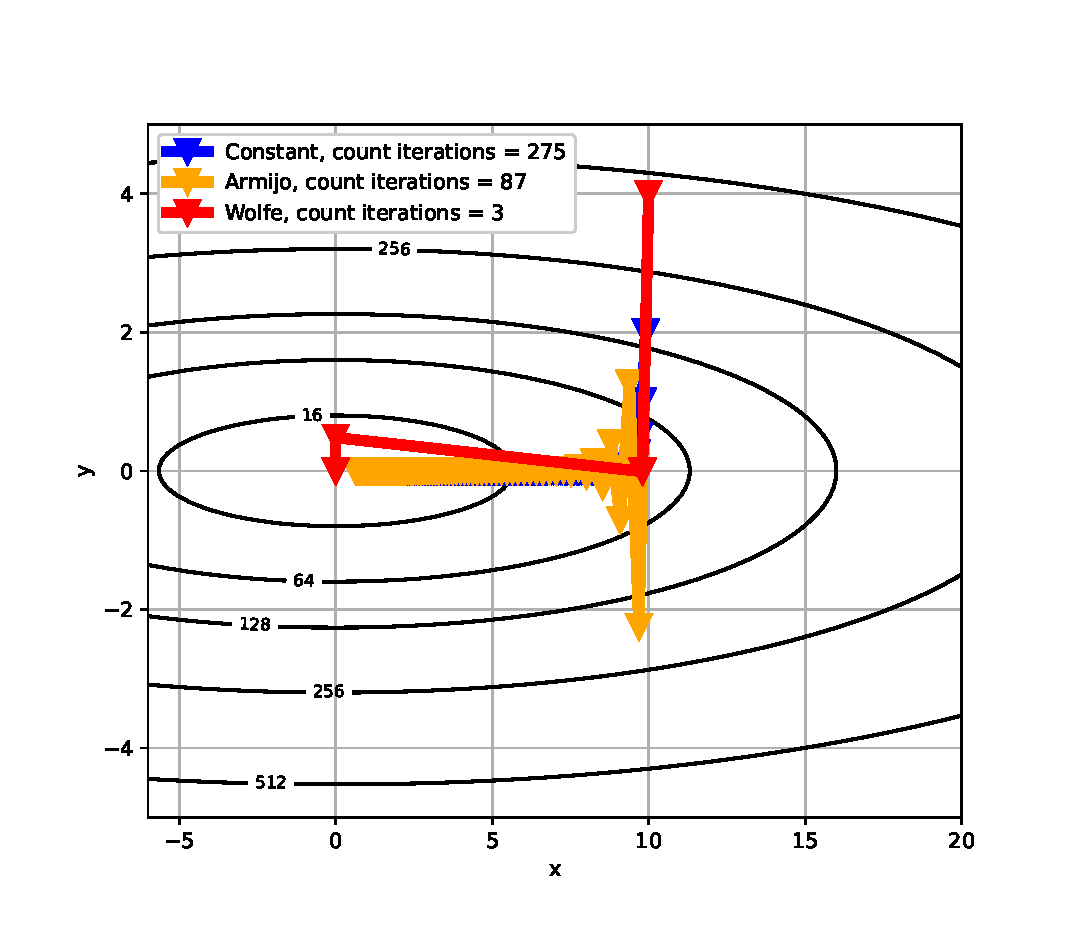
\includegraphics[width=0.5\textwidth]{img/3.1/fig_1}}%
		\hfill % <-- Seperation
		\subcaptionbox{$X =  \left( \begin{smallmatrix} 1 & 0\\ 0 & 5 \end{smallmatrix}  \right)$, $w_0 = (10.0, 4.0)$}{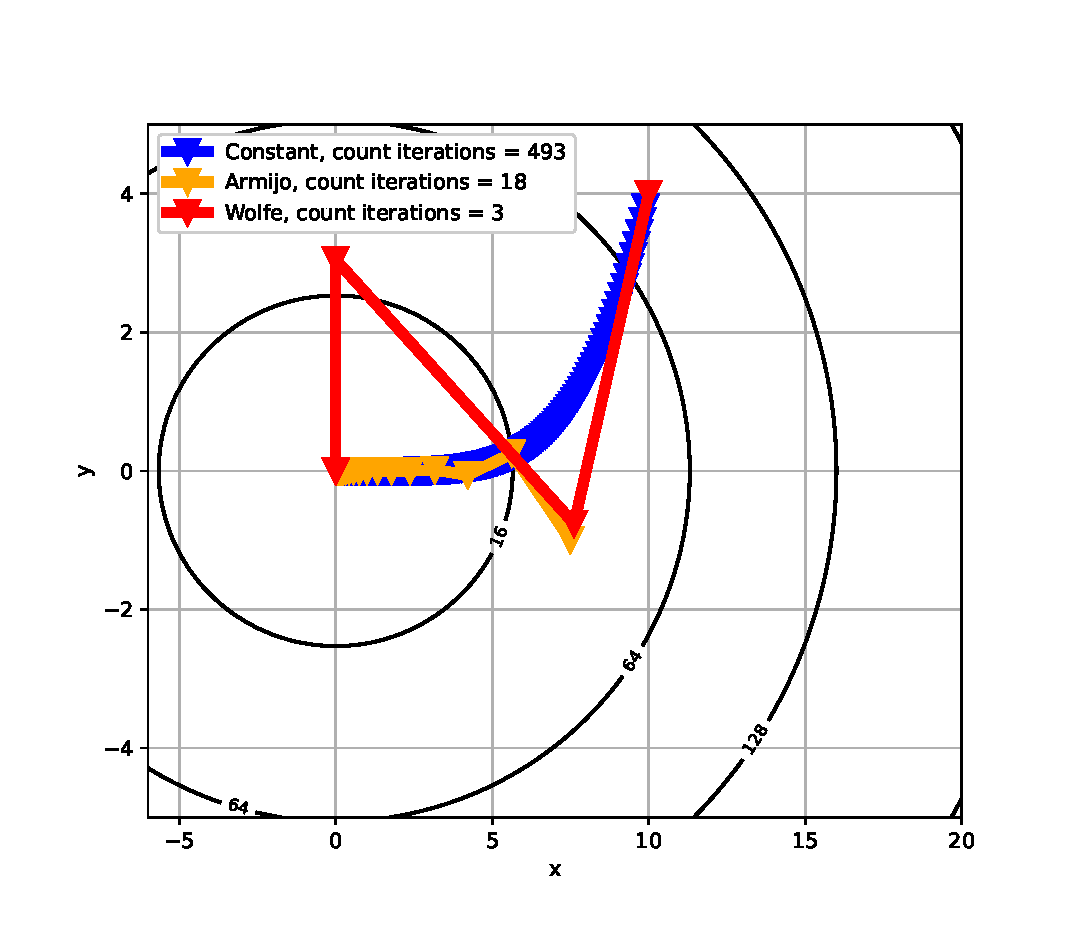
\includegraphics[width=0.5\textwidth]{img/3.1/fig_2}}%
		\caption{Траектория спуска для различных обусловленностей матрицы}
		\label{fig:obyslovlenn}
	\end{figure}
	
	\newpage
	Можно заметить, что, чем ниже обусловленность матрицы, тем больше итераций делает спуск с постоянной длиной шага, а спуску методом Армихо, наоборот, требуется в 3 раза меньше операций.
	Также траектория спуска с постоянным шагом стала более плавной, на Рис.\ref{fig:obyslovlenn} (a), мы видим, как направление спуска резко сменилось на $90^{\circ}$, а на том же рисунке с литерой (b), траектория меняется более плавно. Траектория Армихо в среднем не изменилась, также видны резкие изменения траектории, но ближе к точке минимума траектория становится более плавной и совпадает со спуском с постоянным шагом. Траектория Вульфа стала более криволинейной, каждый шаг делается практически с разворотом на $90^{\circ}$, но благодаря подбору шага этому методу требуется меньше итераций, чем двум другим.
	
	\vspace{1cm}
	
	\begin{figure}[H]
		\centering
		\subcaptionbox{$X =  \left( \begin{smallmatrix} 0.5 & 0\\ 0 & -0.5 \end{smallmatrix}  \right)$, $w_0 = (3.0, -3.0)$}{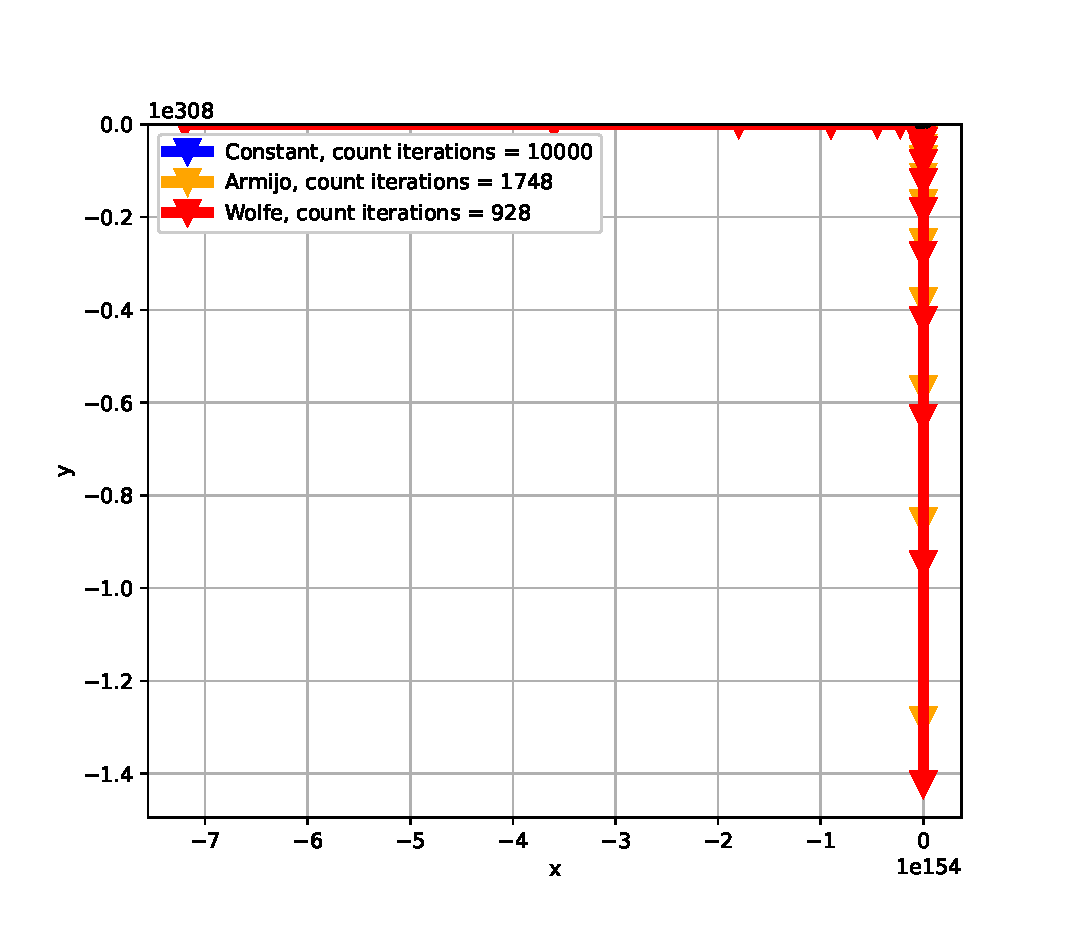
\includegraphics[width=0.5\textwidth]{img/3.1/fig_3}}%
		\hfill % <-- Seperation
		\subcaptionbox{$X =  \left( \begin{smallmatrix} 0.5 & 0\\ 0 & -0.5 \end{smallmatrix}  \right)$, $w_0 = (1.0, 0.0)$}{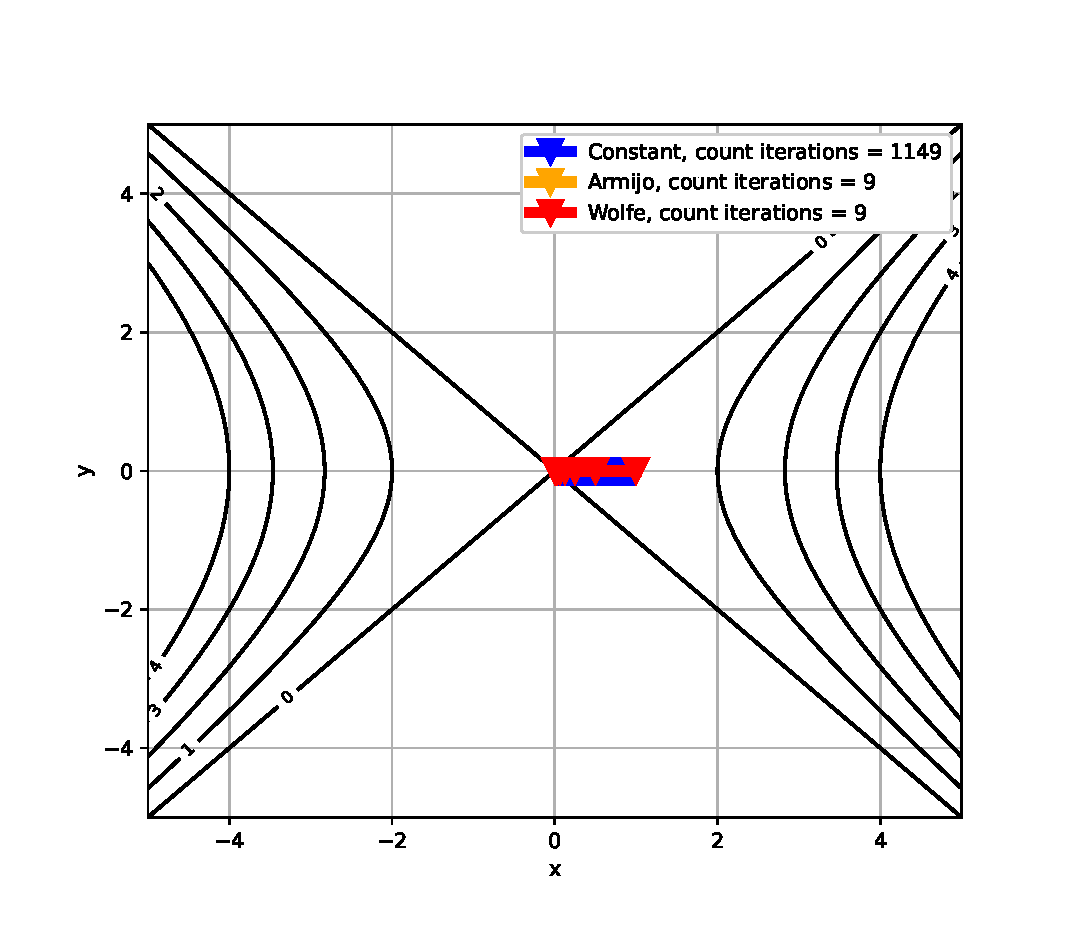
\includegraphics[width=0.5\textwidth]{img/3.1/fig_4}}%
		\caption{Выбор начальной точки}
		\label{fig:start_point}
	\end{figure}
	
	На Рис.\ref{fig:start_point} ищется локальный минимум функции $f(x) = \frac{1}{2}x^2 - \frac{1}{2}y^2$ --- так называемая, седловая функция. Ее особенность заключается в том, что найти ее минимум можно тогда и только тогда, когда начинаем спуск с точки $w_{init} = (1.0, 0.0)$, это можно легко доказать теоретически. Также заметим, что на Рис.\ref{fig:start_point} (a) константный метод дошел до предела итераций, но так и не достиг $-\infty$ по значению функции. Армихо и Вульф достигли этого нижнего предела, сработал критерий останова, причем метод Вульфа снова обогнал другие методы спуска. На Рис. \ref{fig:start_point} (b) все 3 метода сходятся в одну точку, но спуску с постоянным шагом требуется куда больше итераций для этого.
	
	\vspace{2cm}
	\subsection{Зависимость числа итераций градиентного спуска от числа обусловленности и размерности пространства}
	
	Продолжаем работать с той же самой квадратичной функцией. В предыдущем эксперименте мы сделали некоторые предположения о количестве итераций, необходимых для сходимости спуска с разными методами подбора шага. Сейчас мы построим эту зависимость наглядно. Начнем со спуска с постоянной длиной шага. Изобразим 3 варианта графика, каждый соответсвует уникальной константе для выбора длины шага.
	
	\newpage
	
	\begin{figure}[H]
		\centering
		\subcaptionbox{}{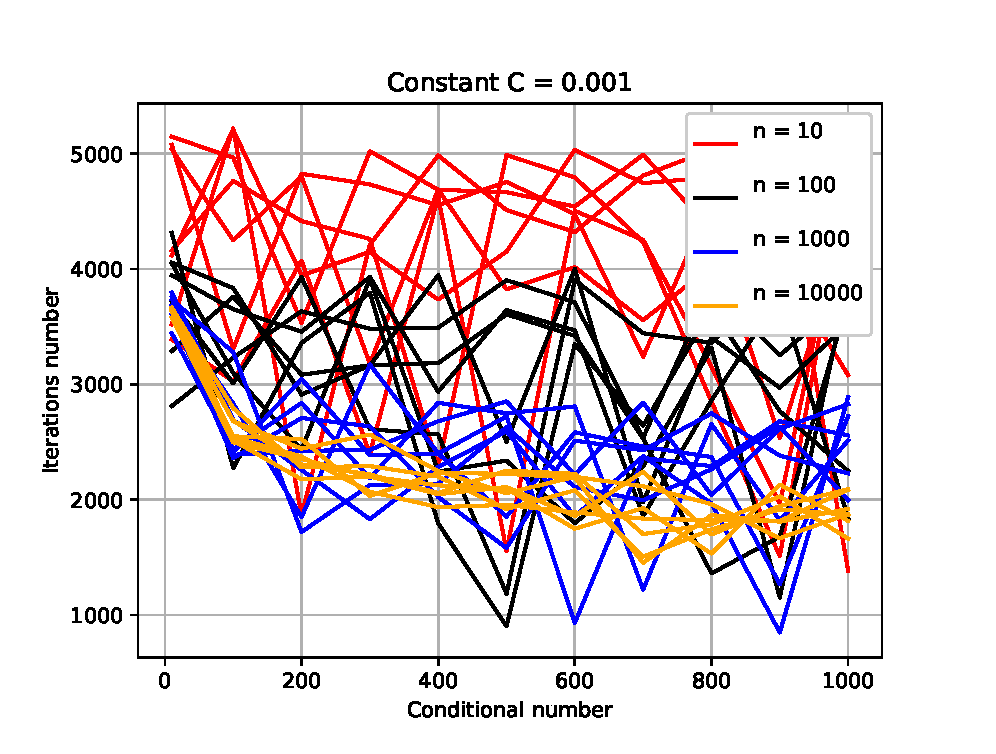
\includegraphics[width=0.5\textwidth]{img/3.2/Constant_0.001}}%
		\hfill % <-- Seperation
		\subcaptionbox{}{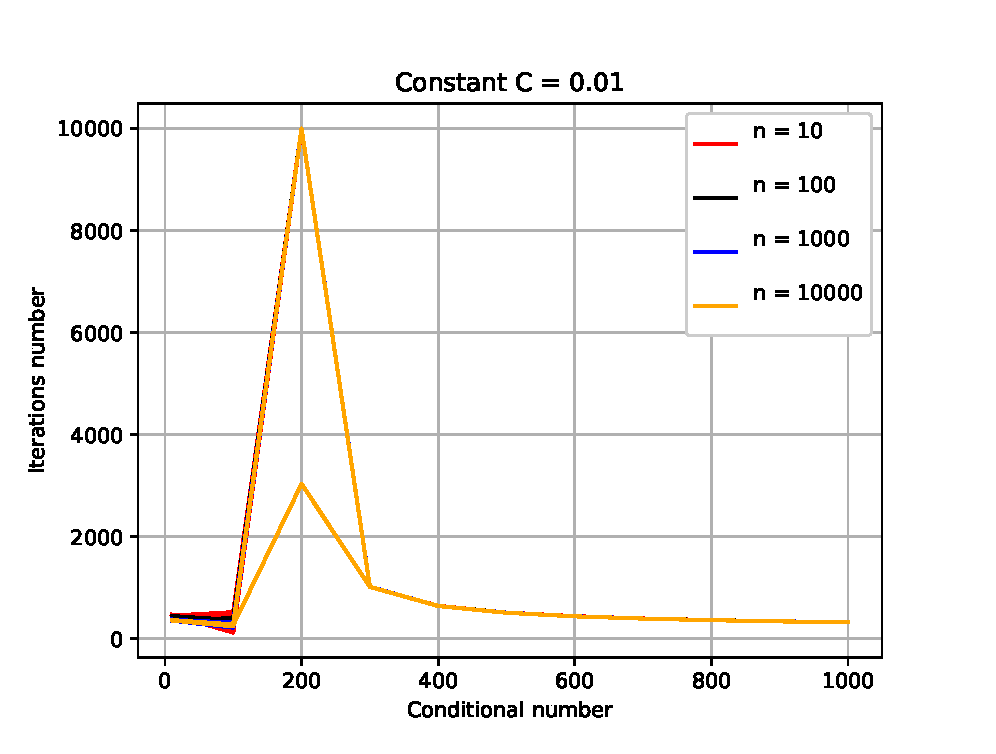
\includegraphics[width=0.5\textwidth]{img/3.2/Constant_0.01}}%
		\\ % <-- Line break
		\subcaptionbox{}{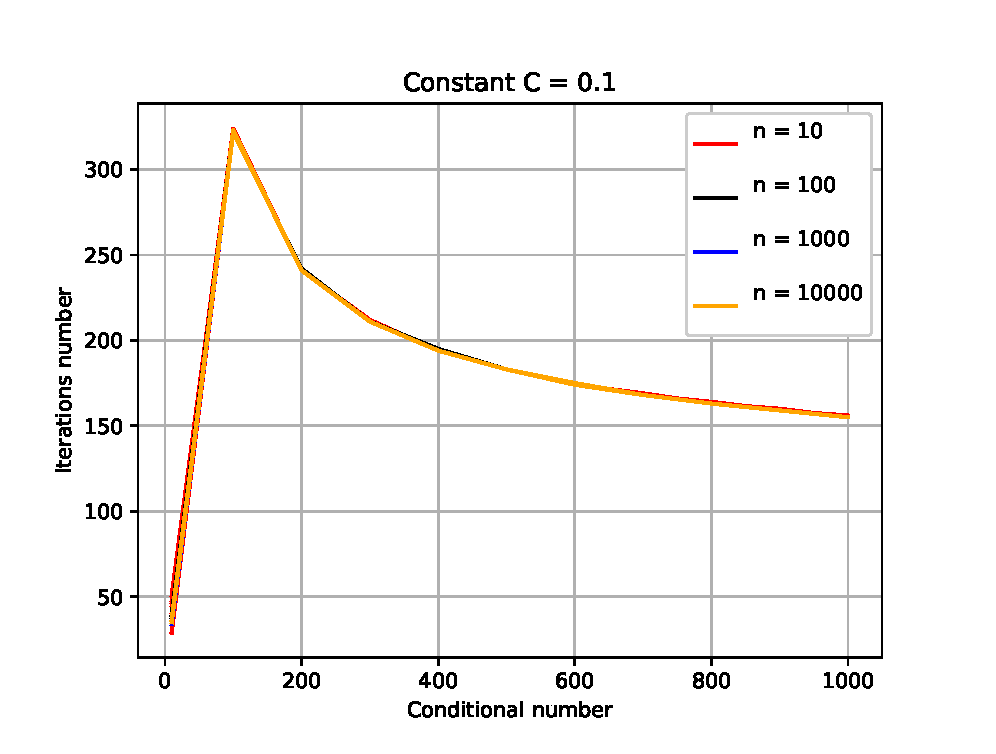
\includegraphics[width=0.5\textwidth]{img/3.2/Constant_0.1}}%
		\hfill % <-- Seperation
		\subcaptionbox{}{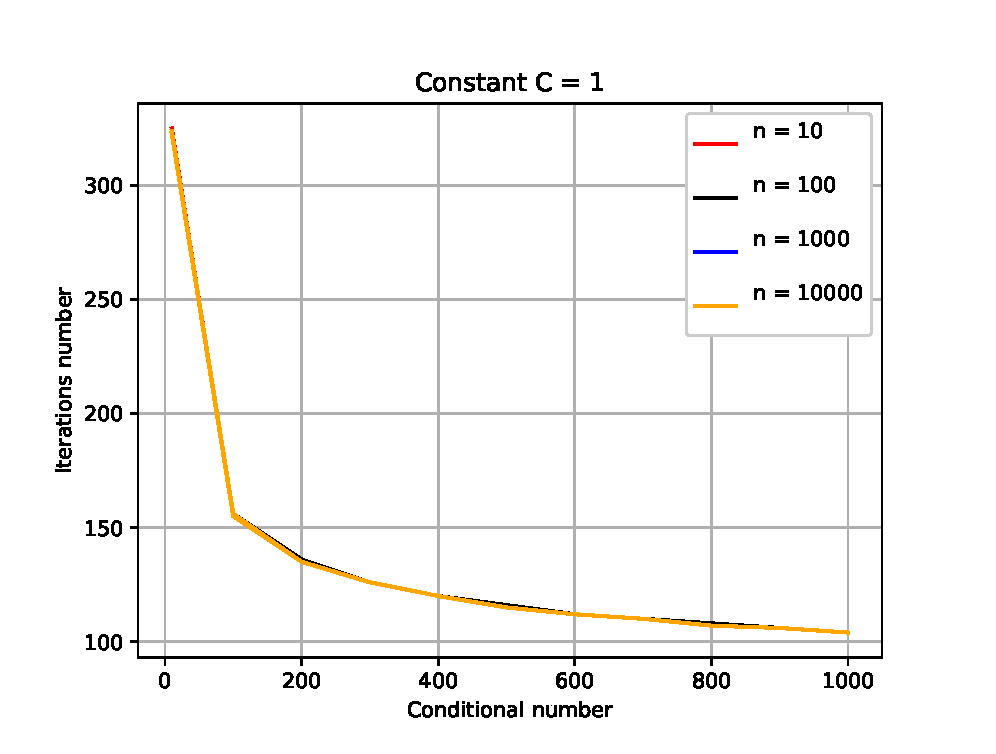
\includegraphics[width=0.5\textwidth]{img/3.2/Constant_1}}%
		\caption{Постоянная длина шага}
		\label{fig:const_alpha}
	\end{figure}

	Посмотрим на Рис.\ref{fig:const_alpha}. Под литерой (а) не прослеживается четкой линейной или квадратичной зависимости. Но мы отчетливо видим, что чем ниже размерность матрицы, тем больше итераций для спуска необходимо провести. Кроме того, с увеличением размерности, падает разброс графиков --- они становятся более скученными, так, например, для размерности $n = 10000$, мы наблюдаем практически гиперболическую зависимость $(f(x) = \frac{1}{x})$, а также очень малую дисперсию количества итераций, по сравнению с другими размерностями. Если мы увеличим константу на порядок --- Рис.\ref{fig:const_alpha}(b) --- ,то заметим, как сильно изменилась ситуация. Мы видим довольно скученный график на обусловленности $k <= 100$ для всех размерностей. Далее, в интервале $100 < k <= 300$ для всех размерностей требуется самое большое значение итераций (даже для $n = 10000$, т.к. на графике только 3 линии из 7). Для $k>300$ значение итераций не столь велико для всех размерностей. Видно, что график выходит на ассимптотику. Продолжаем увеличивать константу --- Рис.\ref{fig:const_alpha}(с)(d) --- видно, что для таких значений $C$ размерность матрицы не имеет значения, влияет лишь обусловленность, но влияет не сильно, разница между максимальным и минимальным значением итераций на двух графиках равна $200$. Также отчетливо прослеживается гиперболическая зависимость, которую мы наблюдали для $C = 0.001$ и $n = 10000$ на Рис.\ref{fig:const_alpha}(a). Также видно, что при $C = 0.1$ и $n \rightarrow \infty$ ассимптотически значения количества итераций больше, чем при $C = 1$ и $n \rightarrow \infty$.
	
	\vspace{1cm}
	Теперь переходим к анализу зависимостей для методов Армихо и Вульфа. 
	
	\newpage
	\begin{figure}[H]
		\centering
		\subcaptionbox{}{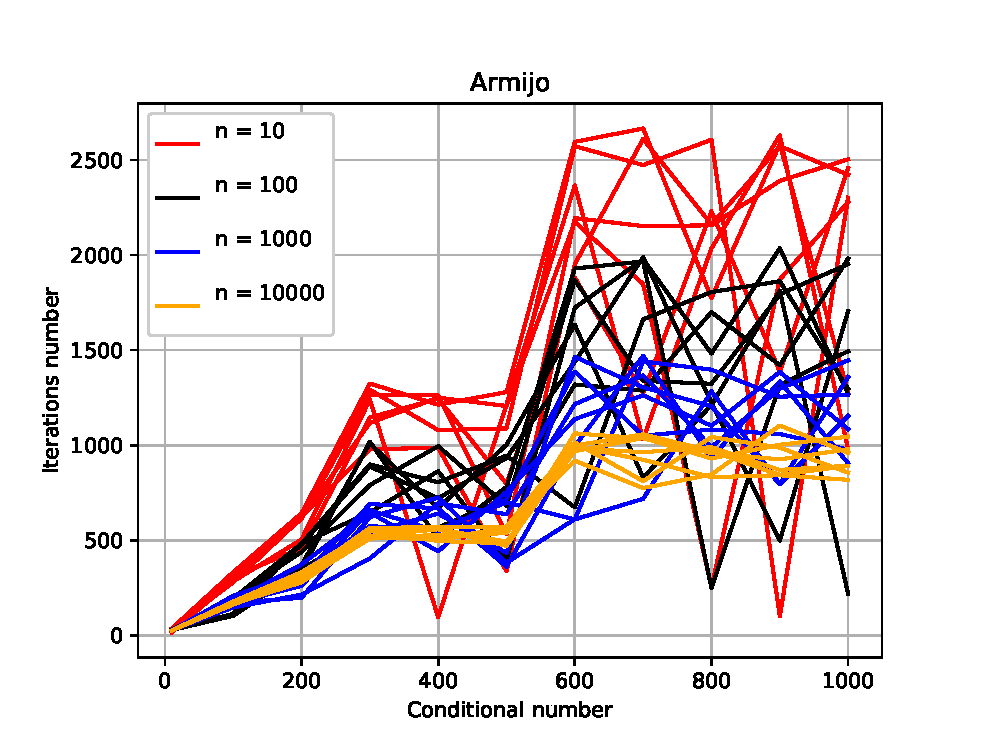
\includegraphics[width=0.5\textwidth]{img/3.2/Armijo}}%
		\hfill % <-- Seperation
		\subcaptionbox{}{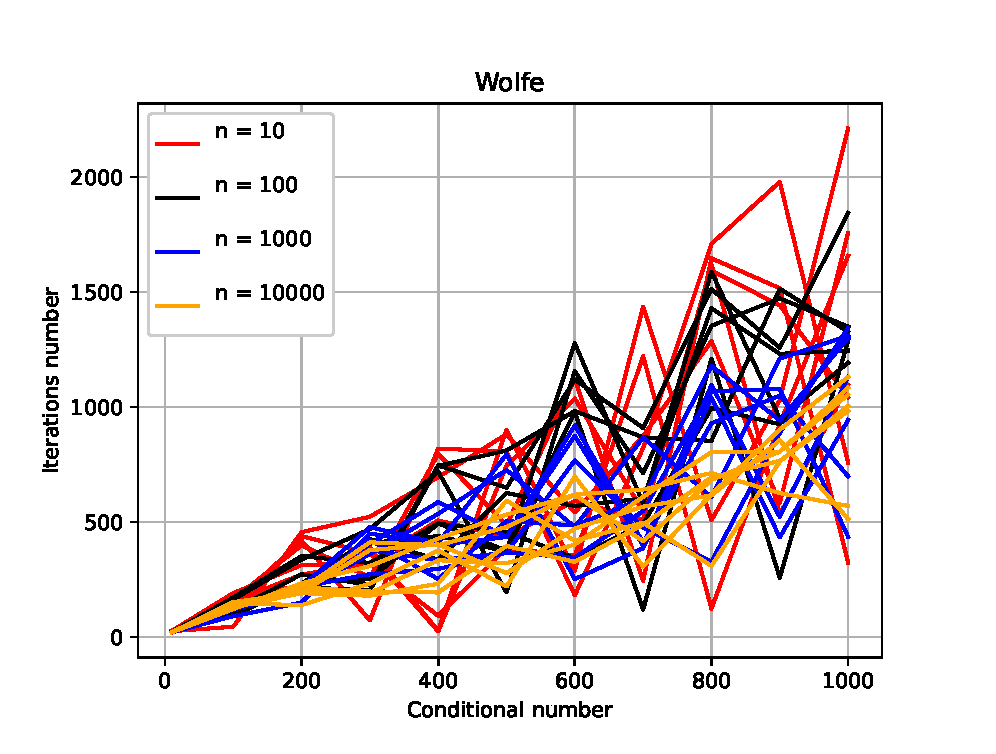
\includegraphics[width=0.5\textwidth]{img/3.2/Wolfe}}%
		\caption{Армихо и Вульф}
		\label{fig:armijo_wolfe}
	\end{figure}
	
	На Рис.\ref{fig:armijo_wolfe}(a), который соответствует условию Армихо, мы наблюдаем четкую линейную зависимость в интервале $0 < k <= 300$, далее график становится похож на Рис.\ref{fig:const_alpha}(a), но с меньшим разбросом и меньшей верхней границей количества итераций. При $n = 10000$ график выходит на ассимптотику. На Рис.\ref{fig:armijo_wolfe}(b) --- условие Вульфа, видна линейная зависимость на всем интервале обусловленности. Дисперсия количества итераций повышается линейно с увеличением обусловленности функции. На всей области определения разброс всех кривых сильнее, чем у метода Армихо.
	
	\vspace{1cm}
	\subsection{Точность оптимизации в реальных задачах для метода Ньютона}
	
	Как мы знаем, на практике в задачах классификации, нас редко интересует только минимизация логистической функции потерь. Существует довольно много различных метрик, которые в той или иной степени измеряют качество решения задач. В этом эксперименте, мы попробуем установить зависимость, между точностью $\epsilon$ \footnote{Вспомним критерий останова --- $\|\nabla f(x_k) \|^2 \leq \epsilon \|\nabla f(x_0) \|^2$.} приближения логистической функции и самых распространенных метрик машинной классификации.
	
	Обучать модель будем на реальных данных. В первом сете содержится информация о \textbf{наличии диабета}. Во втором о \textbf{заболевании сердца}.
	
	\begin{figure}[H]
		\centering
		\subcaptionbox{Стандартный}{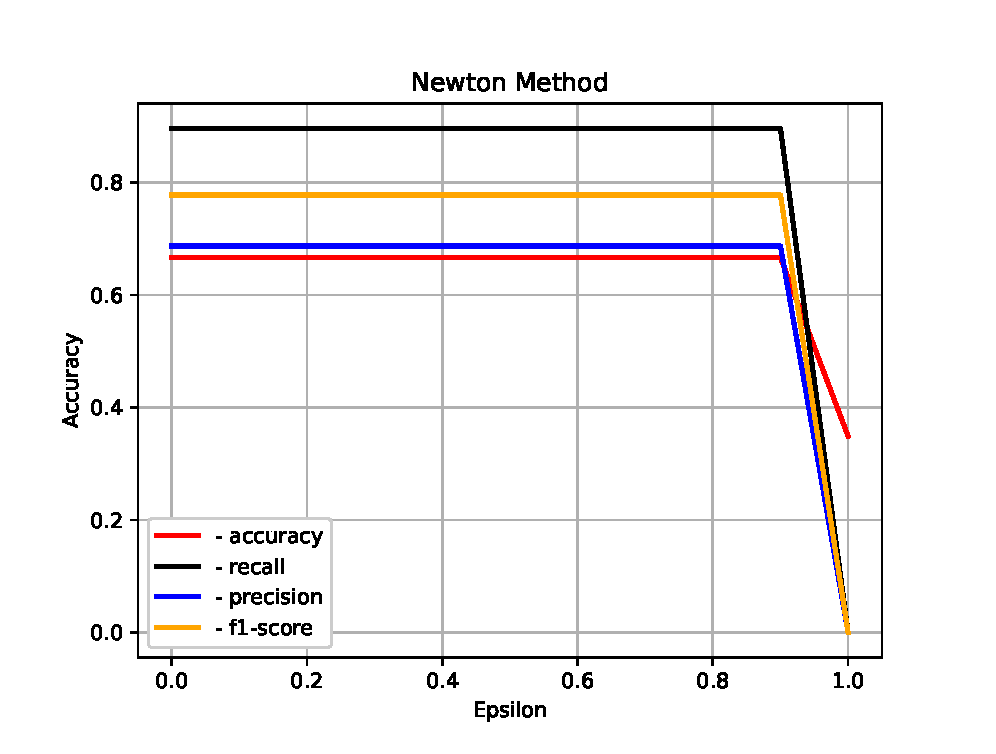
\includegraphics[width=0.5\textwidth]{img/3.3/diabetes}}%
		\hfill % <-- Seperation
		\subcaptionbox{Масштабированный}{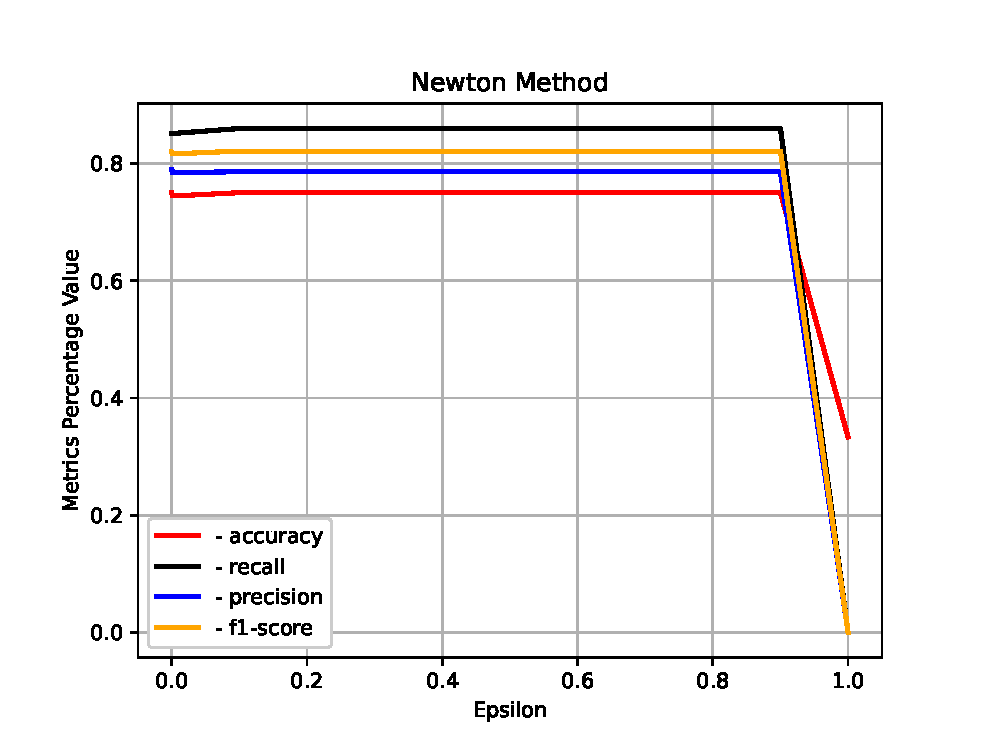
\includegraphics[width=0.5\textwidth]{img/3.3/diabetes_scale}}%
		\caption{Диабет}
		\label{fig:diabet}
	\end{figure}
	
	\newpage
	Рис.\ref{fig:diabet}(a) --- обучение модели на ''сырых'' данных, тот же рисунок под литерой (б) --- данные отмасштабированы на отрезок [-1, 1]. Заметим, что зависимость всех метрик на диапазоне [0.1, 1] линейна от $\epsilon$, это легко понять на уровне интуиции, чем меньше отношение $\frac{\|\nabla f(x_k) \|^2 }{\|\nabla f(x_0) \|^2}$, тем ближе мы к точке минимума функции. Очевидно, что $\epsilon$ практически не оказывает влияния на метрики, только \textit{accuracy}  увеличивается при $\epsilon \neq 1$, ведь $\epsilon = 1$ соответствует случайному угадыванию весов при признаках, соотвественно доля верных ответов вполне может быть в районе 50\%.
	
	Куда больший интерес представляет Рис.\ref{fig:diabet}(b) --- с  отмасштабированными признаками. Во-первых, отчетливо видно, что даже при самом плохом приближении --- $\epsilon \approx 0.9$ --- все метрики, за исключением полноты, оказываются выше примерно на 10 процентных пунктов, относительно метрик на неотмасштабированных данных. Кроме того, при $\epsilon \approx 10^{-8}$ заметны небольшие изменения --- повысилась доля верных ответов, упала точность, выросла полнота. У нас появилась гипотеза --- метод Ньютона показывает себя лучше на отмасштабированных данных, а от точности приближения практически не зависит. 
	
	Проведем этот же эксперимент на других данных.
	
	\vspace{1.5cm}
	\begin{figure}[H]
		\centering
		\subcaptionbox{Стандартный}{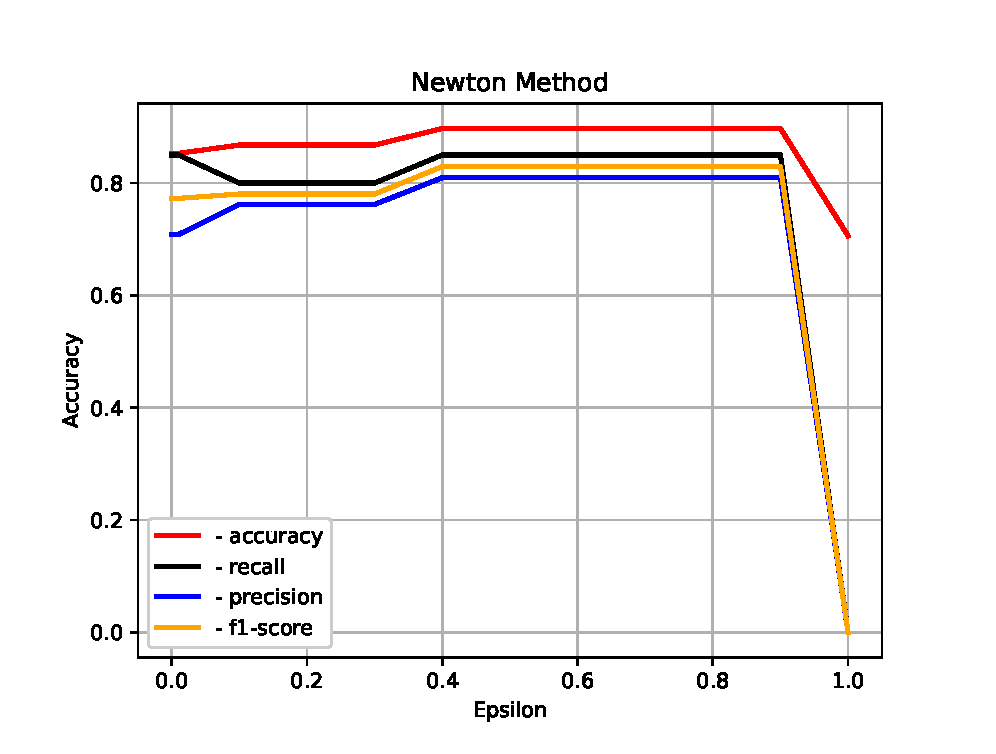
\includegraphics[width=0.5\textwidth]{img/3.3/heart}}%
		\hfill % <-- Seperation
		\subcaptionbox{Масштабированный}{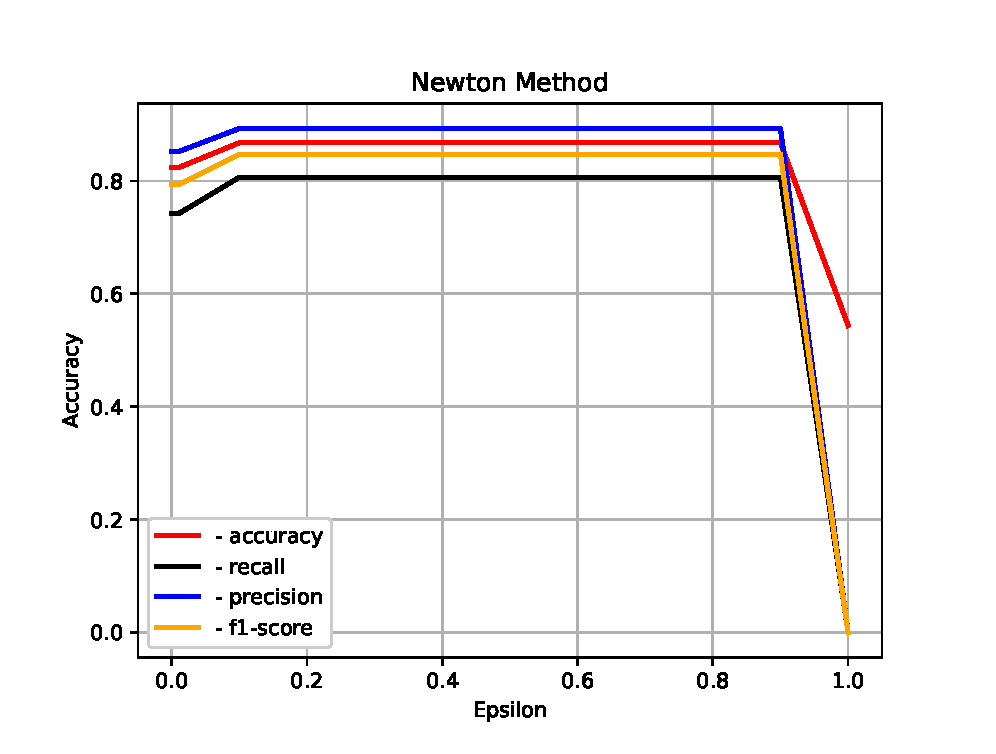
\includegraphics[width=0.5\textwidth]{img/3.3/heart_scale}}%
		\caption{Заболевания сердца}
		\label{fig:heart}
	\end{figure}
	
	Посмотрев на Рис.\ref{fig:heart} заметим, что наша гипотеза подтвердилась на половину --- метод Ньютона не всегда ведет себя эффективнее на масштабированных данных. В этом случае, разница между метриками на двух сетах меньше, чем в данных о диабете. Но при этом, у масштабированных данных, точность и f-мера выше, чем у стандартных. В этом случае масштабированные данные более устойчивы к изменениям точности приближения.
	
	По итогам эксперимента мы точно установили, что практически все метрики обучения не зависят от точности приближения $\epsilon$, а необходимость масштабирования данных необходимо проверять каждый раз эксперементально.  
	
	\newpage
	\subsection{Сравнение методов на реальной задаче логистической регрессии}
	
	В предыдущем эксперименте мы обучались на небольших наборах данных. В каждом было примерно по 800 наблюдений и 15 признаков. Сейчас же мы попробуем увеличить размер выборки как по наблюдениям, так и по признакам. Из-за того, что мой домашний компьютер не может вместить в себя матрицу размером $10^6 \times 10^6$, будем обучаться только на 2 средних сетах. Размер первого будет порядка 50000 наблюдений и 300 признаков, второй имеет размер 72000 на 21000.
	
	
	\begin{figure}[H]
		\centering
		\subcaptionbox{}{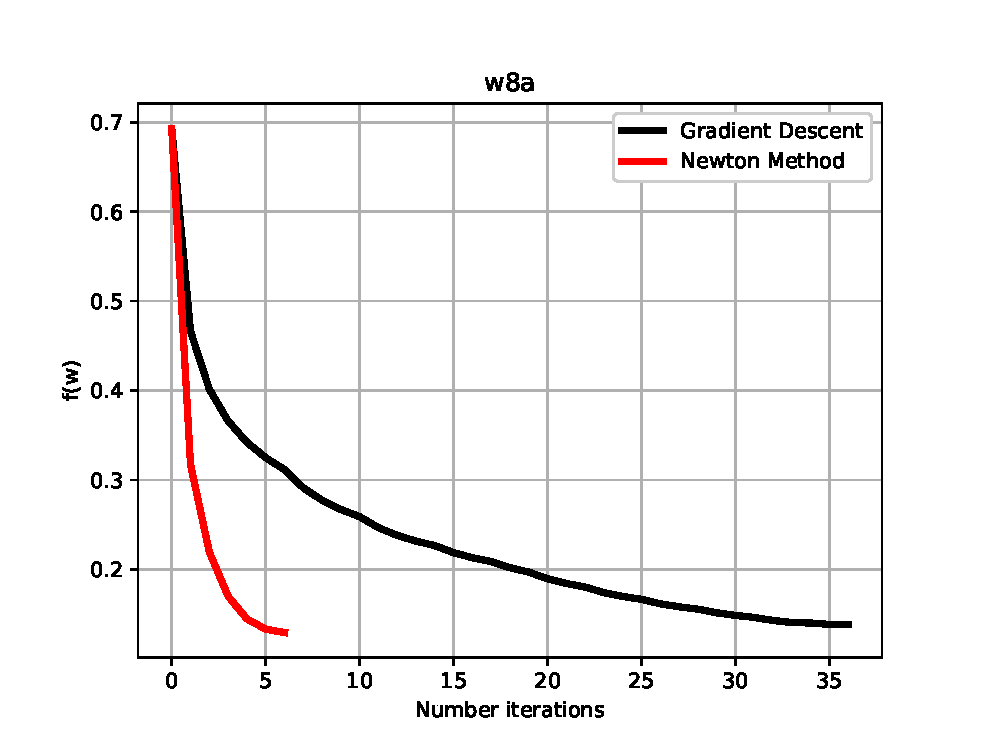
\includegraphics[width=0.5\textwidth]{img/3.4/w8a_func_vs_iter}}%
		\hfill % <-- Seperation
		\subcaptionbox{}{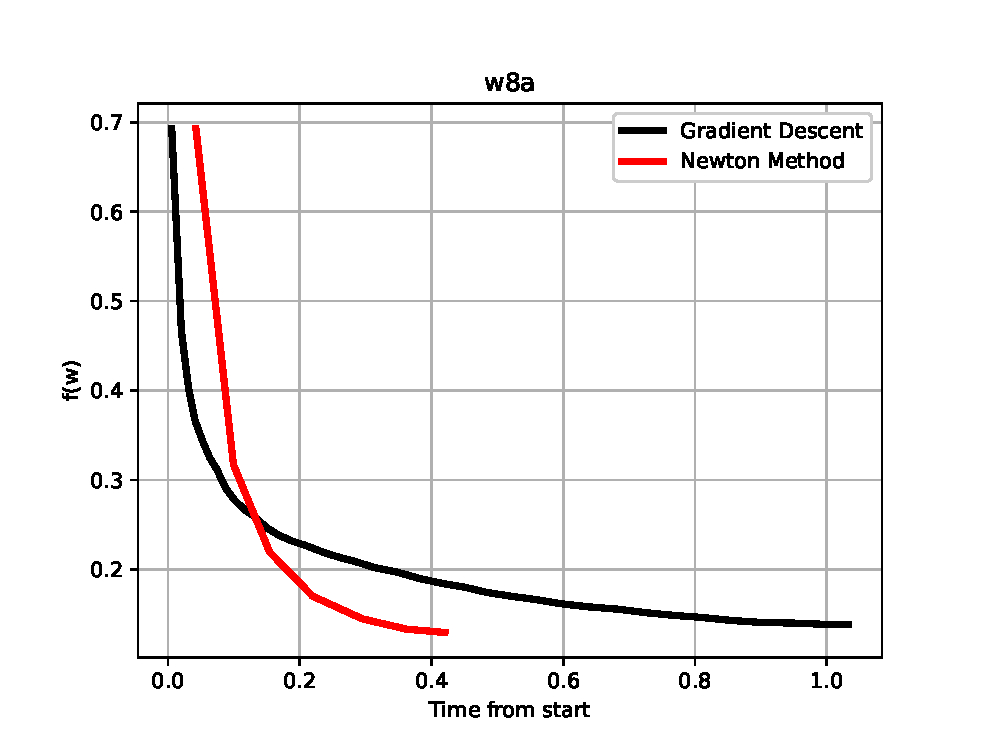
\includegraphics[width=0.5\textwidth]{img/3.4/w8a_func_vs_time}}%
		\hfill % <-- Seperation
		\subcaptionbox{}{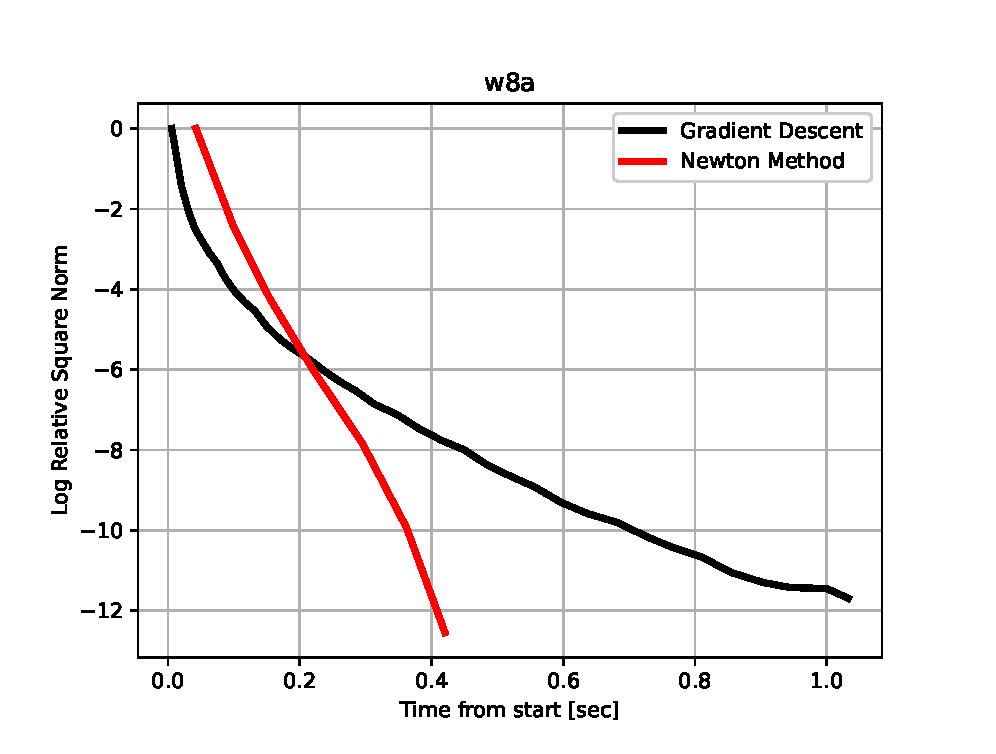
\includegraphics[width=0.5\textwidth]{img/3.4/w8a_rel_sq_grad}}%
		\caption{}
		\label{fig:w8a}
	\end{figure}
	
	На Рис.\ref{fig:w8a} использовался набор данных $w8a$. Здесь четко прослеживается превосходство метода Ньютона с точки зрения инженерной задачи --- за более меньшее количество итераций и меньшее время мы получаем лучшие результаты, как по функционалу ошибки, так и по логарифму относительной нормы градиента. Метод Ньютона сошелся в 2 раза быстрее и сделал в 7 раз меньше итераций по сравнению с градиентным спуском.
	
	Вполне естественно предположить, что на больших объемах данных у метода Ньютона могут возникнуть вычислительные трудности в операциях разложения Холецкого $A = L L^T$ и решении СЛАУ $Ax = b$.
	
	\begin{figure}[H]
		\centering
		\subcaptionbox{}{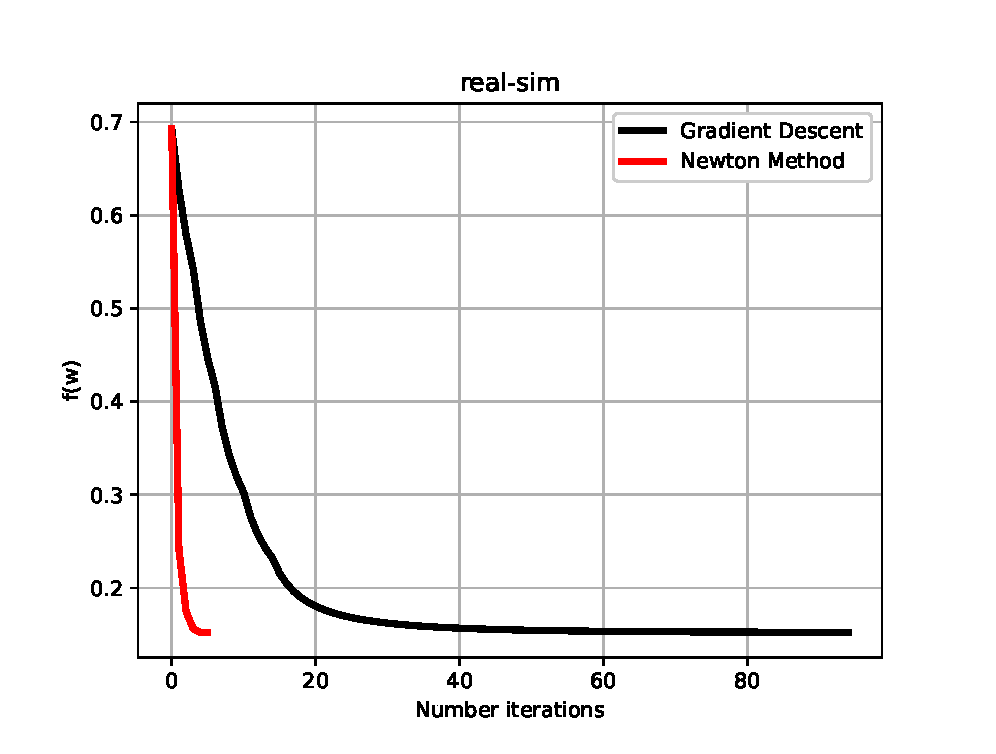
\includegraphics[width=0.5\textwidth]{img/3.4/real-sim_func_vs_iter}}%
		\hfill % <-- Seperation
		\subcaptionbox{}{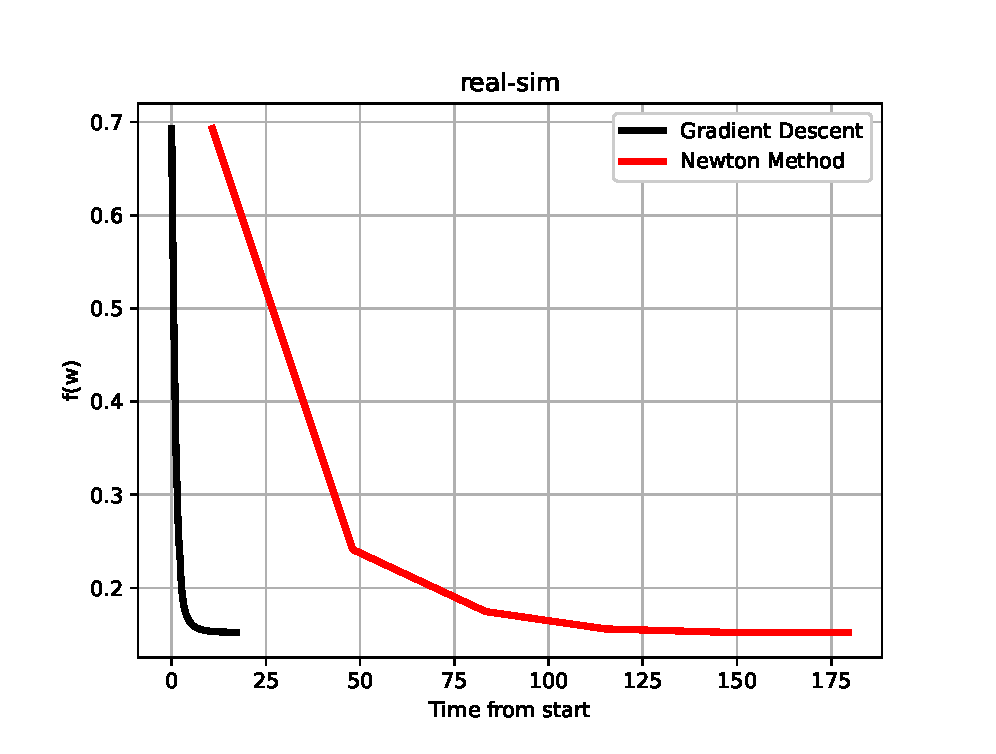
\includegraphics[width=0.5\textwidth]{img/3.4/real-sim_func_vs_time}}%
		\hfill % <-- Seperation
		\subcaptionbox{}{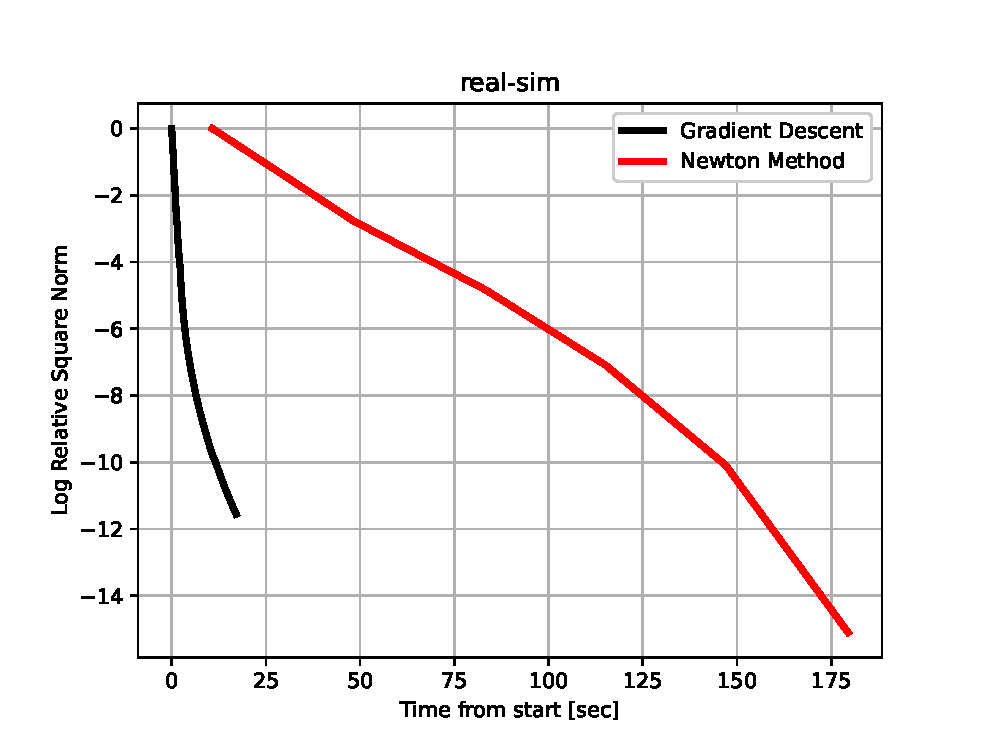
\includegraphics[width=0.5\textwidth]{img/3.4/real-sim_rel_sq_grad}}%
		\caption{}
		\label{fig:real-sim}
	\end{figure}
	
	Наша гипотеза подтвердилась. На Рис.\ref{fig:real-sim} видно, что при размерах матрицы данных порядка $70000 \times 20000$ элементов, метод Ньютона сильно проигрывает градиентному спуску. Градиентный спуск находит локальный минимум в 7 раз быстрее, но тратя при этом в 14 раз больше итераций. Также стоит обратить внимание на то, что Рис.\ref{fig:real-sim}(с) говорит о том, что точность у Ньютоновского метода в 1.5 раза выше, чем у градиентного спуска.
	
	В результате, мы выяснили, что метод Ньютона отлично показывает себя на небольших объемах данных ($50000 \times 1000$ элементов). При увеличении размерности данных, мы получим более долгое время выполнения алгоритма Ньютона, также нам потребуется очень много памяти для хранения матрицы данных, так как разложение Холецкого и решение СЛАУ занимают $O(n^2)$ памяти. 
	
	\vspace{1cm}
	\subsection{Оптимизация вычислений в градиентном спуске}
	
	Посмотрим, как зависят количество итераций и время выполнения программы от оптимизированного и стандартного оракула логистической регрессии. В оптимизированном оракуле более эффективно вычисляются матричные проивзедения, так например, при последовательных выховах оракула в одной и той же точке не происходит перерасчета матрицы, а используется та, которая была получена при первом вызове. Обучать модель будем на синтетических данных --- количество наблюдений 10000, количество признаков 8000. 
	
	\newpage
	\begin{figure}[H]
		\centering
		\subcaptionbox{}{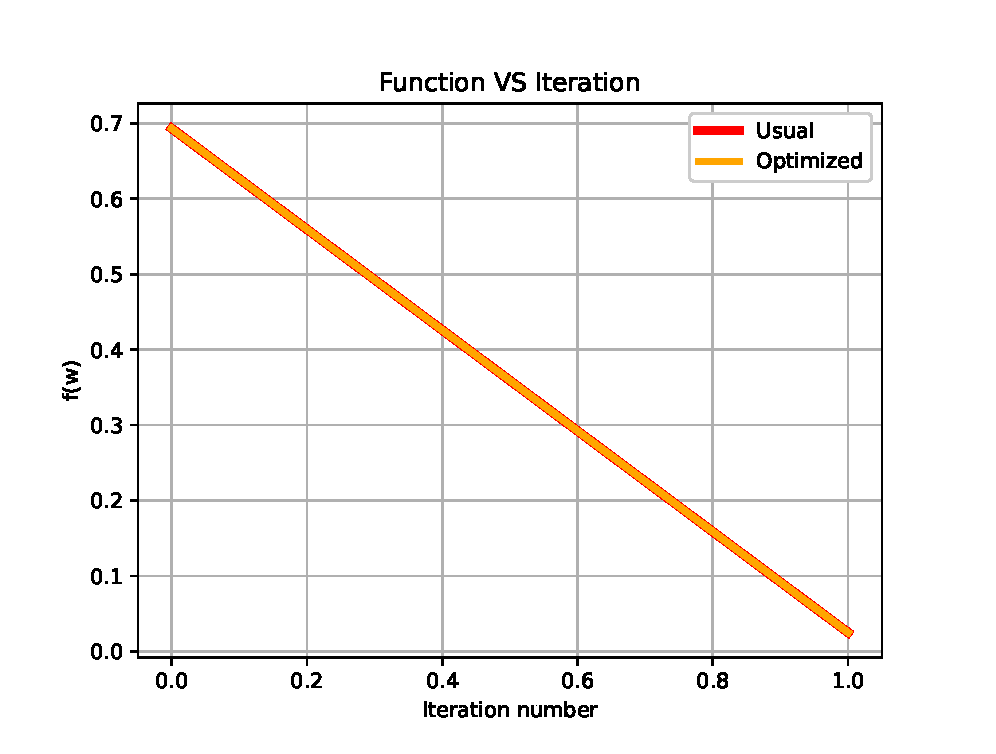
\includegraphics[width=0.5\textwidth]{img/3.5/func_vs_iter}}%
		\hfill % <-- Seperation
		\subcaptionbox{}{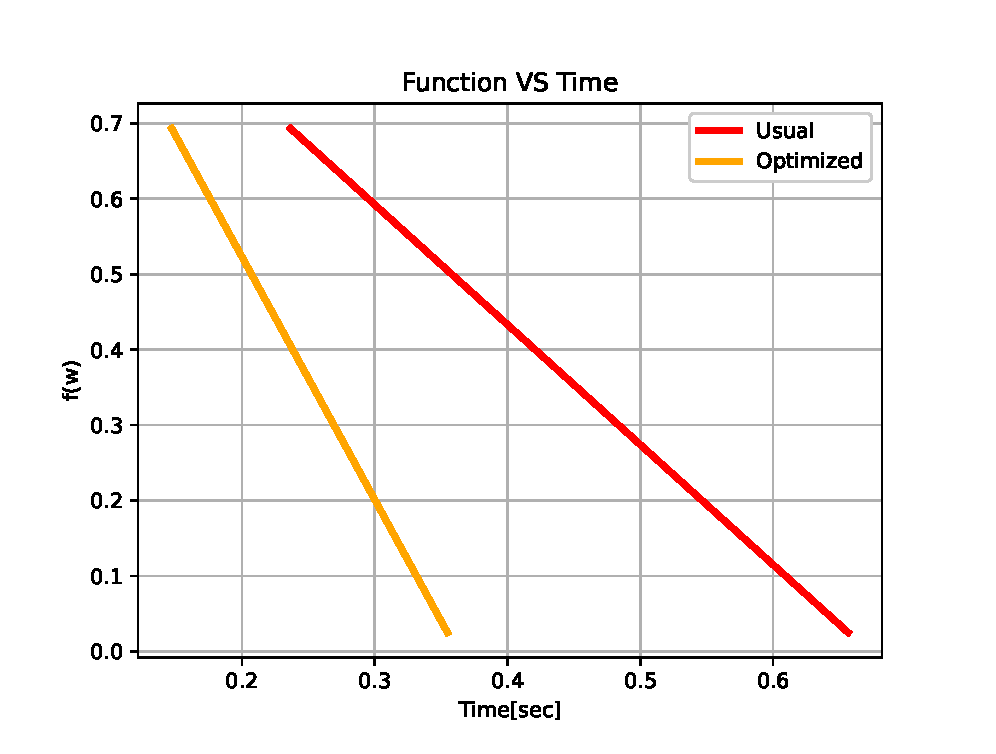
\includegraphics[width=0.5\textwidth]{img/3.5/func_vs_time}}%
		\hfill % <-- Seperation
		\subcaptionbox{}{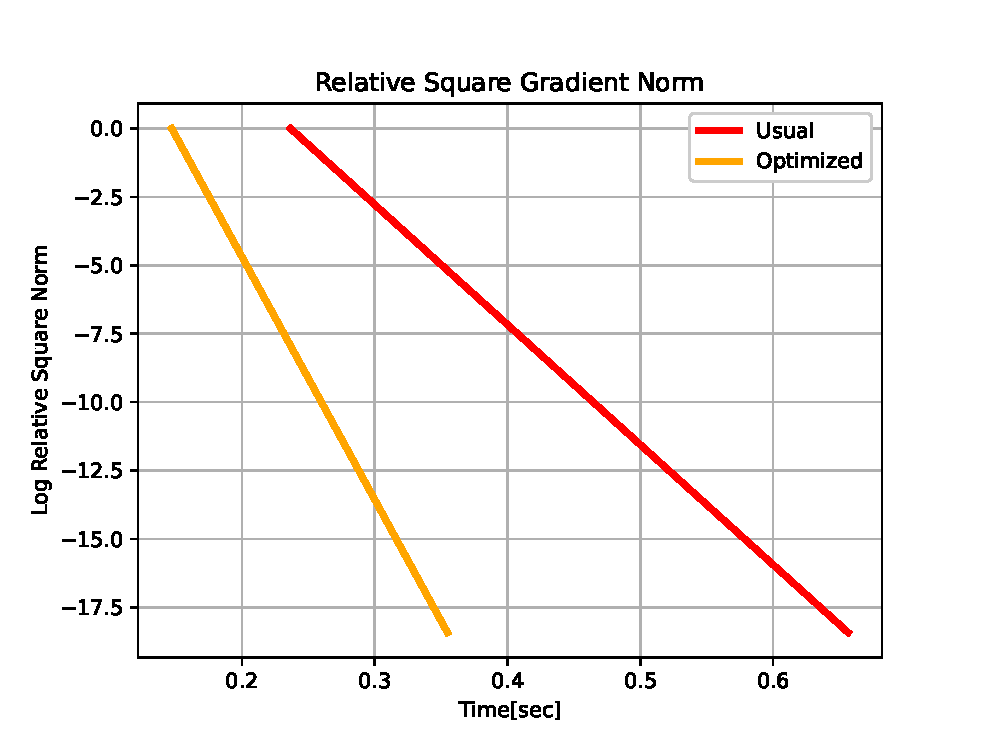
\includegraphics[width=0.5\textwidth]{img/3.5/rel_sq_grad}}%
		\caption{}
		\label{fig:log_reg_opt}
	\end{figure}
	
	На Рис.\ref{fig:log_reg_opt} видно, что оптимизированный оракул справляется быстрее, но при этом, ему требуется то же самое количество итераций --- оно и не удивительно, ведь мы просто храним значения матриц, а не используем дополнительные хитрости для вычислений. Оптимизированный подсчет логистической функции справляется примерно в 2 раза быстрее, не теряя при этом точности в вычислениях.
	
	
	
	
	
	
\end{document}
